%!TEX root = ../thesis.tex
%*******************************************************************************
%****************************** Fourth Chapter *********************************
%*******************************************************************************

\chapter{Marco teórico}

\ifpdf
    \graphicspath{{Chapter4/Figs/}{Chapter4/Figs/PDF/}{Chapter4/Figs/}}
\else
    \graphicspath{{Chapter4/Figs/}{Chapter4/Figs/}}
\fi


\section{Resultados}

\subsection{Implementación}
En principio se intentó utilizar las últimas versiones LTS disponibles de las tecnologías
seleccionadas para llevar adelante el proyecto pero debido a inconsistencias e incompatibilidades
entre versiones de Node, librerías y solidity se tuvo que trabajar en encontrar un conjunto de
versiones que hagan un ecosistema estable para el desarrollo. Por otra parte, se pudo trabajar con
las últimas versiones estables de React y su ecosistema sin problemas.

Se trabajó con el controlador de versiones Git y la plataforma GitHub para almacenar el
repositorio.

\subsection{Pruebas}
Las pruebas realizadas sobre la aplicación constan por un lado de las pruebas manuales que
cualquier
usuario podría hacer en el uso del día a día. Y por otro lado se escribieron tests con Mocha en la
plataforma de Node.js que constaten que la compilación, deploy y métodos del contrato solidity
funcionen correctamente.

Se pospuso para versiones avanzadas el testeo vía código de los componentes React debido a que la
mayoría de ellos depende de conexiones con Ethereum y el contrato para recibir los datos y poder
renderizarse correctamente. Esta tarea es lo que dificulta un poco su testeo total. Una vía de escape
para este problema, es mockear las llamadas a Ethereum y usar dummy data para trabajar durante los
tests automatizados.

\subsection{Versionado}
Como se dijo en la sección de \textit{implementación}, se utilizó Git como sistema de versionado.
Para llevar un control ordenado del código de una manera lo más similar posible a proyectos reales
y de cualquier envergadura (ya sea tanto proyectos pequeños como corporativos a gran escala) se
decidió utilizar parcialmente git flow. 

De manera resumida, git flow propone el uso de ciertas ramas con reglas características de cada
una. Para el desarrollo de la aplicación se usaron las ramas \textit{master, develop} y 
\textit{feature}.

\begin{itemize}
	\item Master
	
	Cualquier commit que se encuentre en esta rama debe estar preparado para subir a producción.
	
	\item Develop
	
	Rama en la que está el código que conformará la siguiente versión planificada del proyecto.
	
	\item Feature
	
	Estas ramas se utilizan para desarrollar nuevas características de la aplicación que, una vez
	terminadas, se incorporan a la rama develop.
	
	Características:
	\begin{itemize}
		\item Se originan a partir de la rama develop.
		\item Se incorporan siempre a la rama develop.
		\item Nombre: cualquiera que no sea master, develop, hotfix-* o release-*
		\begin{wrapfigure}{l}{1\textwidth}
		\centering    
		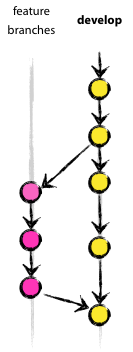
\includegraphics[height=0.3\textheight]{feature_branches}
		\caption[featurebranches]{Diagrama de cómo quedan conformados los commits.}
		\label{fig:feature-branches}
		\end{wrapfigure}
	\end{itemize}

\end{itemize}
